\chapter{Disk Based Index}
\lhead{Chapter 3. \emph{Disk Based Index}} % this is for the header on each page - perhaps a shortened title
\section{Introduction}
Disk Based Inverted Index is our first index libary to serve all \texttt{iZENECloud} products with efficient control of memory consumption together with a high performance. Compared
with other open source solutions such as Lucene \cite{lucene}, the fundamental architecture is similar while we have several extra highlights. As shown in figure \ref{fig:voc1}, basic
inverted index is composed of two parts: vocabulary and posting lists. The vocabulary contains all indexed terms and its pointer to cooresponding posting list. The major design issues
are discussed in the following section. Within \texttt{SF1}, corresponding component of this disk based inverted index is \texttt{IndexManager}.
\begin{figure}[htp]
\centering
\centerline{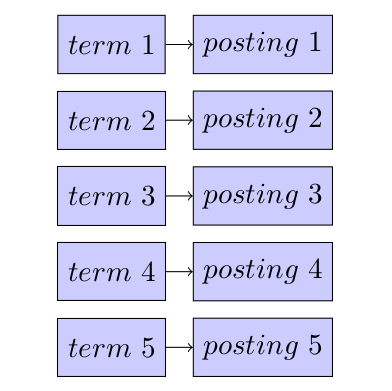
\includegraphics[width=.4\textwidth]{Figures/voc1.png}}
\caption{Inverted Index}\label{fig:voc1}
\end{figure}

\section{Design Issues}
\subsection{Vocabulary Design}
In order to reduce memory consumption, we've adopted an engineering trick of \texttt{Sparse Binary Search}. As we can see from figure \ref{fig:voc1}, the vocabulary itself 
is nothing more than a hash map, since we store term ids within the vocabulary, each entry of the vocabulary has a fixed length. During search process, if we do not load any 
entries of the vocabulary into memory, for each query, we will have to need $O(log|Voc|))$ disk accesses to locate posting lists, while when sparse binary search is applied, 
we could reduce the disk accesses to $O(1)$ instead of $O(log|Voc|))$, as seen in figure \ref{fig:voc2}.

\begin{figure}[h!]
\centerline{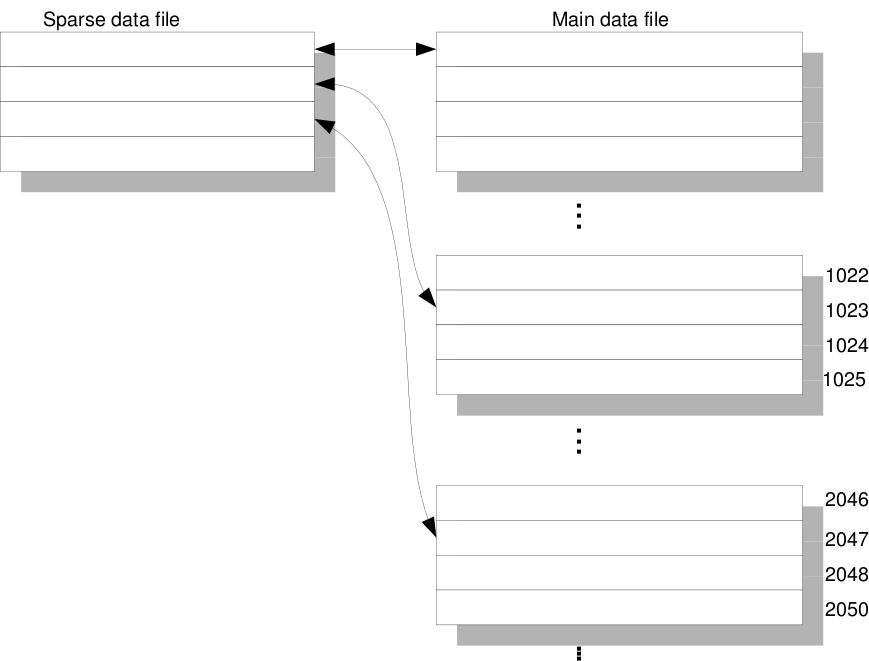
\includegraphics[width=0.6\textwidth]{Figures/voc2.png}}
\caption{Sparse Binary Search}\label{fig:voc2}
\end{figure}

Via storing each 512th entry of the vocabulary data in memory, and then ensuring that the initial delta value of the binary search algorithm is a power of 512, all comparisons required for the binary search will use the data
available in main memory. This optimization requires $O(log|Voc|/512))$ main memory usage.

When using the sparse data described above, the first phrase of the binary search algorithm can determine two 512 entry areas of the vocabulary where the record searched for may reside. Since the overhead of positioning
the disk heads for a read operation is high relative to the time a disk transfer, it will pay off to buffer these 1023 entries when the delta gets below the value of 512. 

\subsection{Index Construction}\label{indexCon}
IndexManager is designed to support both on-line indexing, which is mainly used for real-time search, as well as traditional off-line indexing. The user of IndexManager could designate either of these two indexing modes easily 
just by a configuration parameter. The index construction processes for each of these two modes are totally different:
\begin{itemize}
 \item The real-time indexing requires the inverted index for a certain document to be able to search immediately just after that document is indexed. 
 \item The offline indexing could build index for a batch of documents at one time for a much faster indexing speed.
\end{itemize}

The real-time indexing has a much higher design complexity than the offline one. In order to make the design of both two indexing modes into an overall integrity, we introduce a new concept---\texttt{Index Barrel},
which means the index of a batch of documents. As a result, for the overall indices, we might have multiple index barrels, each of which contain cooresponding documents:
\begin{itemize}
 \item For the offline mode, index for all documents to be indexed will be encapsulated into a single index barrel.
 \item The index construction process for on-line mode will be discussed in the following sub section \ref{indexcon-merge}.
\end{itemize}

In following subsections, we will describe the detailed index construction process for both two modes respectively.

\subsubsection{Off-line Index Construction} \label{indexcon-offline}
Off-line index means the index for the documents could not be searched during indexing. In this case, we could design a very efficient process to make the batch indexing extremely fast:
The inputs of IndexManager is a series of documents, each of which is nothing more than a series of terms, each of which is composed of both term id and term position. As a result, we could look on the 
batch inputs as a series of such kinds of data structures:
\begin{lstlisting}[language=C]
struct Term
{
    uint32_t docId;
    uint32_t termId;
    uint32_t termPosition;
};
\end{lstlisting}
And we need all of these inputs to be sorted according to the priority of \texttt{termId},\texttt{docId} and \texttt{termPosition}, the key design issue is how could we sort the data inputs efficiently ?

\begin{figure}[h!]
\centerline{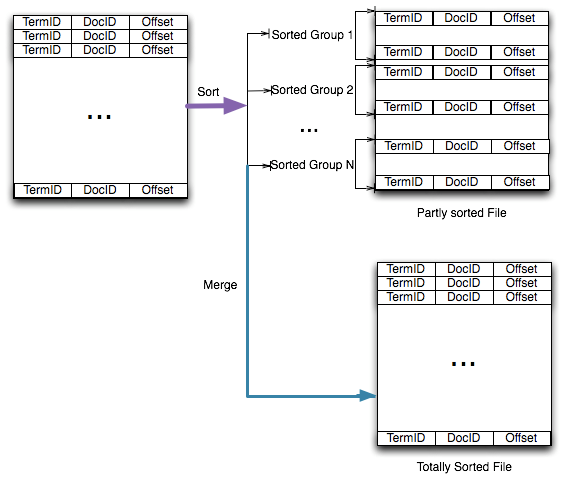
\includegraphics[width=0.6\textwidth]{Figures/izene_sort.png}}
\caption{Offline Index Sorting Process}\label{fig:indexcon-sort}
\end{figure}


Figure \ref{fig:indexcon-sort} has illustrated the sorting process adopted by IndexManager---it's an improved version for \texttt{merge-sort} process that is frequently used in external sorting algorithms:
\begin{itemize}
 \item Firstly, IndexManager will create a memory buffer, say 100M, to accumulate the inputed data.
 \item When the memory buffer is full, a memory sort will be performed for those contained data, and the results will be written to an intermediate file.
 \item The above steps will be continuously looped until there are no documents to be indexed. As a result, the intermediate file is a partly sorted file.
 \item A final merge sort will be performed based on the previously mentioned intermediate file.
\end{itemize}

Such merge sort based process is extremely efficient. For each batch off-line indexing process, a single index barrel is generated, while if we have several index operations, 
eg: we index 1M documents, 100k documents, and 10k documents sequentially, we then have 3 index barrels. How to manage these three index barrels have closely relation with the
on-line index construction mode, and we will discuss this issue in the next sub section.


\subsubsection{Merge Based Index Construction} \label{indexcon-merge}
During past years, great advances have been achieved to build an off-line index, which could not provide query service during the process of index construction. However, with the boom of the web pages' count number, 
to provide search ability during indexes construction has been more and more urgent, therefore how to maintain on-line index is the current research hotspot on indexing problems. There are three kinds of index construction
method: In-place, Re-build, and Re-merge\cite{lester2004pvr}. For In-place update strategy, documents are accumulated in main memory. Then, once main memory is exhausted, the existing on-disk index is combined with 
the in-memory index by appending each posting list from the in-memory index to the corresponding list in the on-disk index; The Re-build algorithm constructs a new index from the current entire collection; For the Re-merge 
update strategy, once main memory is exhausted, a merge event is triggered, and the entire on-disk index is read sequentially and merged with the in-memory index, then written to a new location to form a new on-disk index
that immediately replaces the old one. According to the experiments of \cite{lester2004pvr}, in most cases, Re-merge strategy would perform better than the other two approaches. 

\begin{figure}[h!]
\centerline{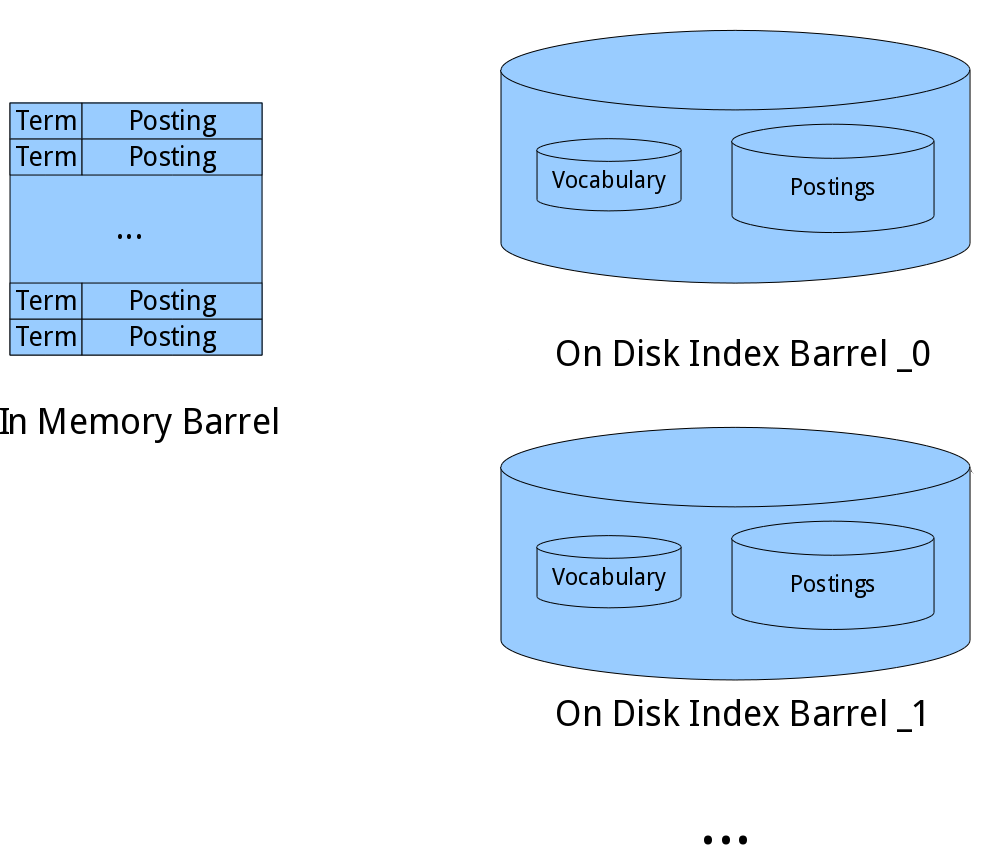
\includegraphics[width=0.4\textwidth]{Figures/barrel1.png}}
\caption{Index Barrels for On-line Indexing}\label{fig:indexcon-barrel1}
\end{figure}

Figure \ref{fig:indexcon-barrel1} shows the on-line indexing process: Unlike offline indexing mode, there's no sorting process for a batch of documents, instead, inverted index is built for each document as soon as that 
document is pass to IndexManager. There's a memory pool maintained by IndexManager, as soon as index for documents has used up that memory pool, all of the index data will be flushed to disk to form an on disk
index barrel, named start from $_0$, $_1$,...,etc, and then the memory pool could contain index for new documents, obviously, the in-memory index is another index barrel.  All of the on disk index barrels as well as 
the in-memory index barrel could be searched start from scratch, so we could provide real-time search utilities in this indexing mode.

The key design issue for this kind of index construction is how we manage these index barrels: because in this kind of indexing mode, we might generate much more index barrels than offline mode: as soon as the memory
pool is used up, we are going to generate a new index barrel. Given a 128M memory pool, we can only index 10k documents approximately. As a result,for a given 5M corpus, we might generate hundreds of index barrels. 
We can not keep the number of index barrels large, or else the search performance will be affected. We also can not merge those index barrels frequently, or else the indexing performance will be affected. The Dynamic 
Balancing Tree algorithm \cite{guo2007eli} is used for one of the index merging policy, which provides an index merging algorithm that supports on-line index maintenance. 
\par
DBT\cite{guo2007eli} index construction strategy is a kind of Re-merge algorithm and performs the best among all available schemes.  A DBT is an m-way tree, each node of which is a sub-index. The tree is divided into $H$ layers from bottom to top. At layer $k$, the number of nodes is either zero, or is less than m. Let $\mathbf{E}_{k,j}$ be the capacity of node $j, 0\leq j<m-1$, at layer $k, 0\leq k<H$, a constraint of the number of documents in one node of layer $k$ is given by:
\begin{equation}
c^{k}\leq \epsilon_{k,j}<c^{k+1}
\end{equation}

When the size of each node in layer $k$ satisfy the above equation, the tree is balanced. When the number of nodes in the layer $k$ is equal to or greater than $m$, a merge event is triggered, resulting a new sub-index. The newly created sub-index will be placed into layer $k+1$. If the tree is balanced and a sub-index merge operation is only performed on one layer, the efficiency of merging process can be guaranteed.   According to the experiments in \cite{guo2007eli}, choosing the param value of $m=c=3$ offers better indexing performance. \par

In the implementation, the index is organized into several barrels. One barrel refers to one node in the DBT tree. When constructing the index, the postings will be built up in memory at first, when the memory has been exhausted, these postings will be flushed to one barrel, the layer of which in the DBT tree could be computed by the above equation according to the document number that have been indexed in this barrel. If the number of barrels of a certain layer satisfy the merge condition described above, these barrels will be merged together to form a new barrel, and the old barrels will be deleted. Therefore, merge operation has been limited within several barrels since it is an expensive process, and the total barrels could be controlled because too many barrels will effect the query performance. What's more, all of the barrels could be merged into one monad manually to provide better query performance.


IndexManager provides flexible encapsulation so that different kinds of merge policies could be implemented easily. Except for DBT merge policy, IndexManager also has other merge policies, such as multi-way merge, 
which is used by Lucene\cite{lucene}, and optimize-merge, which is used to merge all index barrels into single index barrel for best index search performance. Different kinds of index merge algorithm is shared by both online-indexing
and off-line index, and the user of IndexManager could config to choose the suitable merge algorithm. Figure \ref{fig:indexcon-barrel2} gives a simple graph show for these three different kinds of merge policies.

\begin{figure}[h!]
\centerline{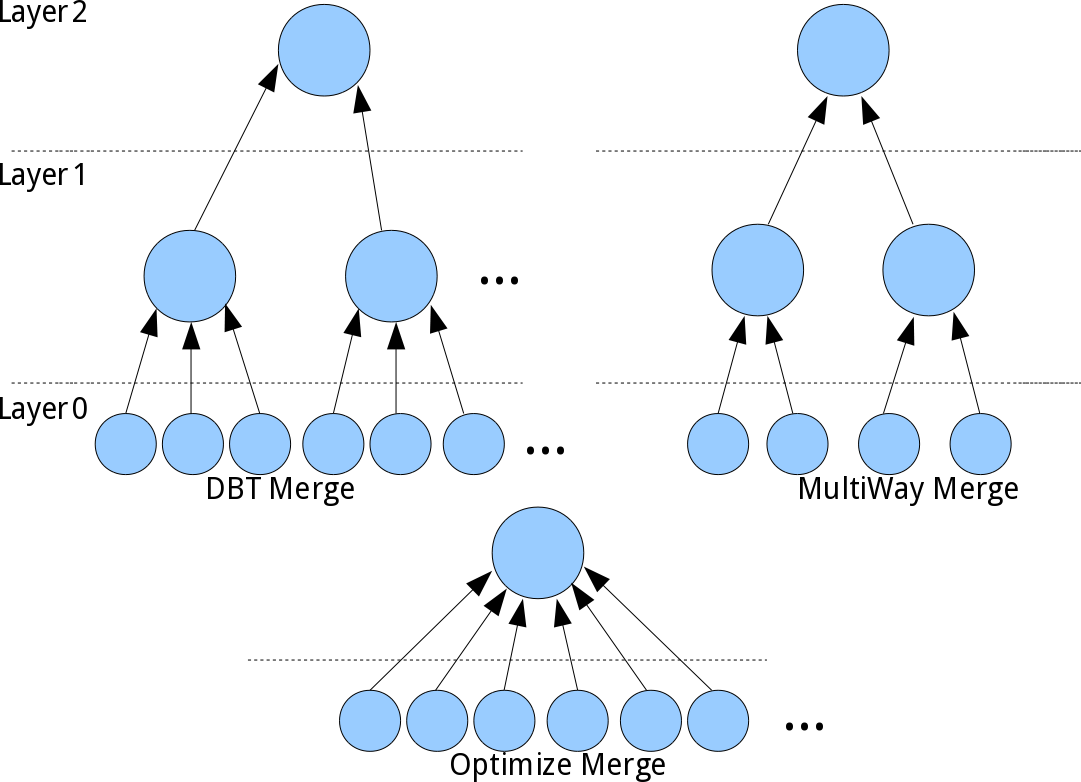
\includegraphics[width=0.6\textwidth]{Figures/barrel2.png}}
\caption{Index Barrels Merge Policies}\label{fig:indexcon-barrel2}
\end{figure}


\subsection{Index Compression}
Compressioin is a very effective solution to struggle with disk IO. There exists a trade off between the compressibility and decoding speed. Higher compression ratio would always lead to slower decoding, if it is too slow, then query performance will be effected. D-gap together with variable length are adopted to compress the index, because it is very fast to decode, and can reduce the index size to about $\frac{1}{2}$ to $\frac{1}{4}$ of the original. It is a mature scheme and has been adopted by most of the existing \texttt{IR} frameworks. This compression solution is the default policy for IndexManager. Besides, we have also implemented the state-of-art index compression scheme, such as \texttt{pForDelta}, a composition of \texttt{pForDelta} and \texttt{S16}, the details could be found in \cite{zukowski2006ssr}, \cite{zhang2008pci},\cite{yan2009inverted},and \cite{yan2009compressing}. These state-of-the-art
compression schemes have also been adopted by the latest \texttt{Google} web search, as a result, our IndexManager has already kept up with the cutting edge of index design area. Since these compression solutions all perform decoding and encoding operations in a batch way, their detailed design within IndexManager is totally different with the variable length solution, we will describe the details in the later section.

\subsection{Index Deletion}
IndexManager uses a bitmap file to indicate the deleted documents. However, if there are too many deleted documents, it will affect the search performance a lot. In that case, IndexManager could utilize the index merger to generate
the new index, within which those delete documents will not appear any more. Another issue is the requirement for supporting \texttt{Document Updating} semantics, in such cases, the updated documents will be assigned with new doc 
ids before they are passed to IndexManager, so that the \texttt{Document Updating} semantics is just a simple composition of \texttt{Document Deletion} and \texttt{Index Document}.

\subsection{B-Tree Index}
When indexing documents, some kinds of data is not suitable to be stored within inverted index, such as date and time, number, etc, because range query is required over vocabulary, 
this is more usual under search filtering. Within \texttt{SF1}, we use B-Tree index for such purpose, the output for any conditional search filtering is a bitmap to be intersected
with results got from inverted index.

\section{Architecture}
Following description for architecture design only focuses on the inverted index parts. There are overall three components for inverted index design:
\begin{itemize}
 \item IndexWriter, which is used to build index---both online and offline.
 \item IndexMerger, which is used to merge index barrels.
 \item IndexReader, which is used to perform search utilities.
\end{itemize}
We will describe each of them in the following sections.


\subsection{IndexWriter}

Figure \ref{indexWriter} shows the hierarchy of IndexWriter of how to form a single barrel index. 

\begin{figure}[h!]
\centerline{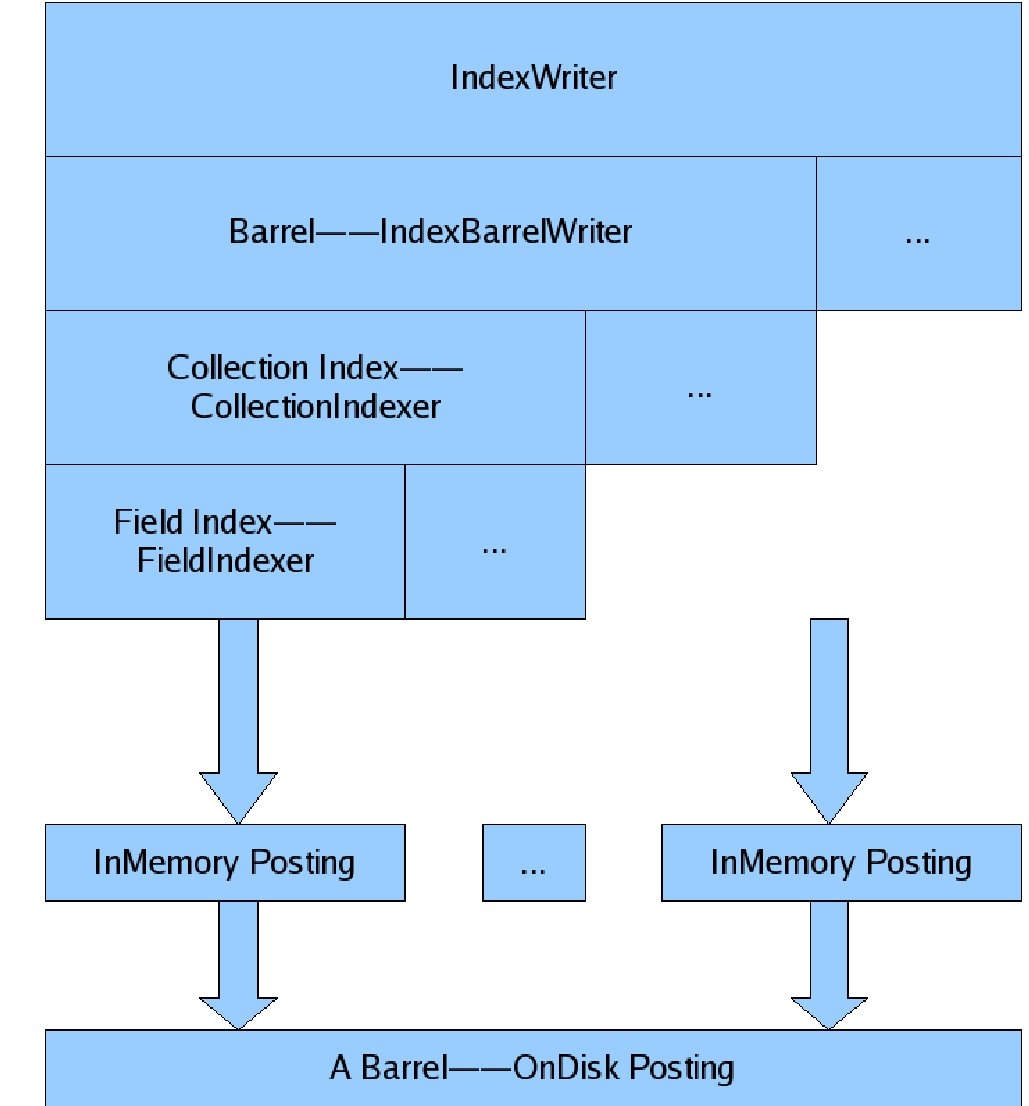
\includegraphics[width=0.4\textwidth]{Figures/indexWriter.jpg}}
\caption{Hierarchy of IndexWriter}\label{indexWriter}
\end{figure}


\par
As has been shown above, IndexBarrelWriter is in charge of flushing index into one barrel. Internally, it contains a serial instances of CollectionIndexer, each of which corresponds to one collection solely. Inside a CollectionIndexer, there are several FieldIndexers, which takes charge of building index within its corresponding Field. After Indexer starts up, the instances of CollectionIndexer and FieldIndexer will be created according to DocumentSchema that have been initialized by the user of IndexManager. In our document model, each document contains several configurable fields, such as \texttt{Title},\texttt{Content},...,etc. Index for each field is independent from each other.  FieldIndexer will build index of one field
of a collection. There are two kinds of posting lists in the system: document-frequency posting and position posting. The former stores document id and frequency of a certain term that has appeared in that document. The latter stores all the term position information of a certain term in the document. 
Suppose we only have general variable length compression scheme, figure \ref{barrelFormat} gives a detailed description of what a single barrel index contains:

\begin{figure}[h!]
\centerline{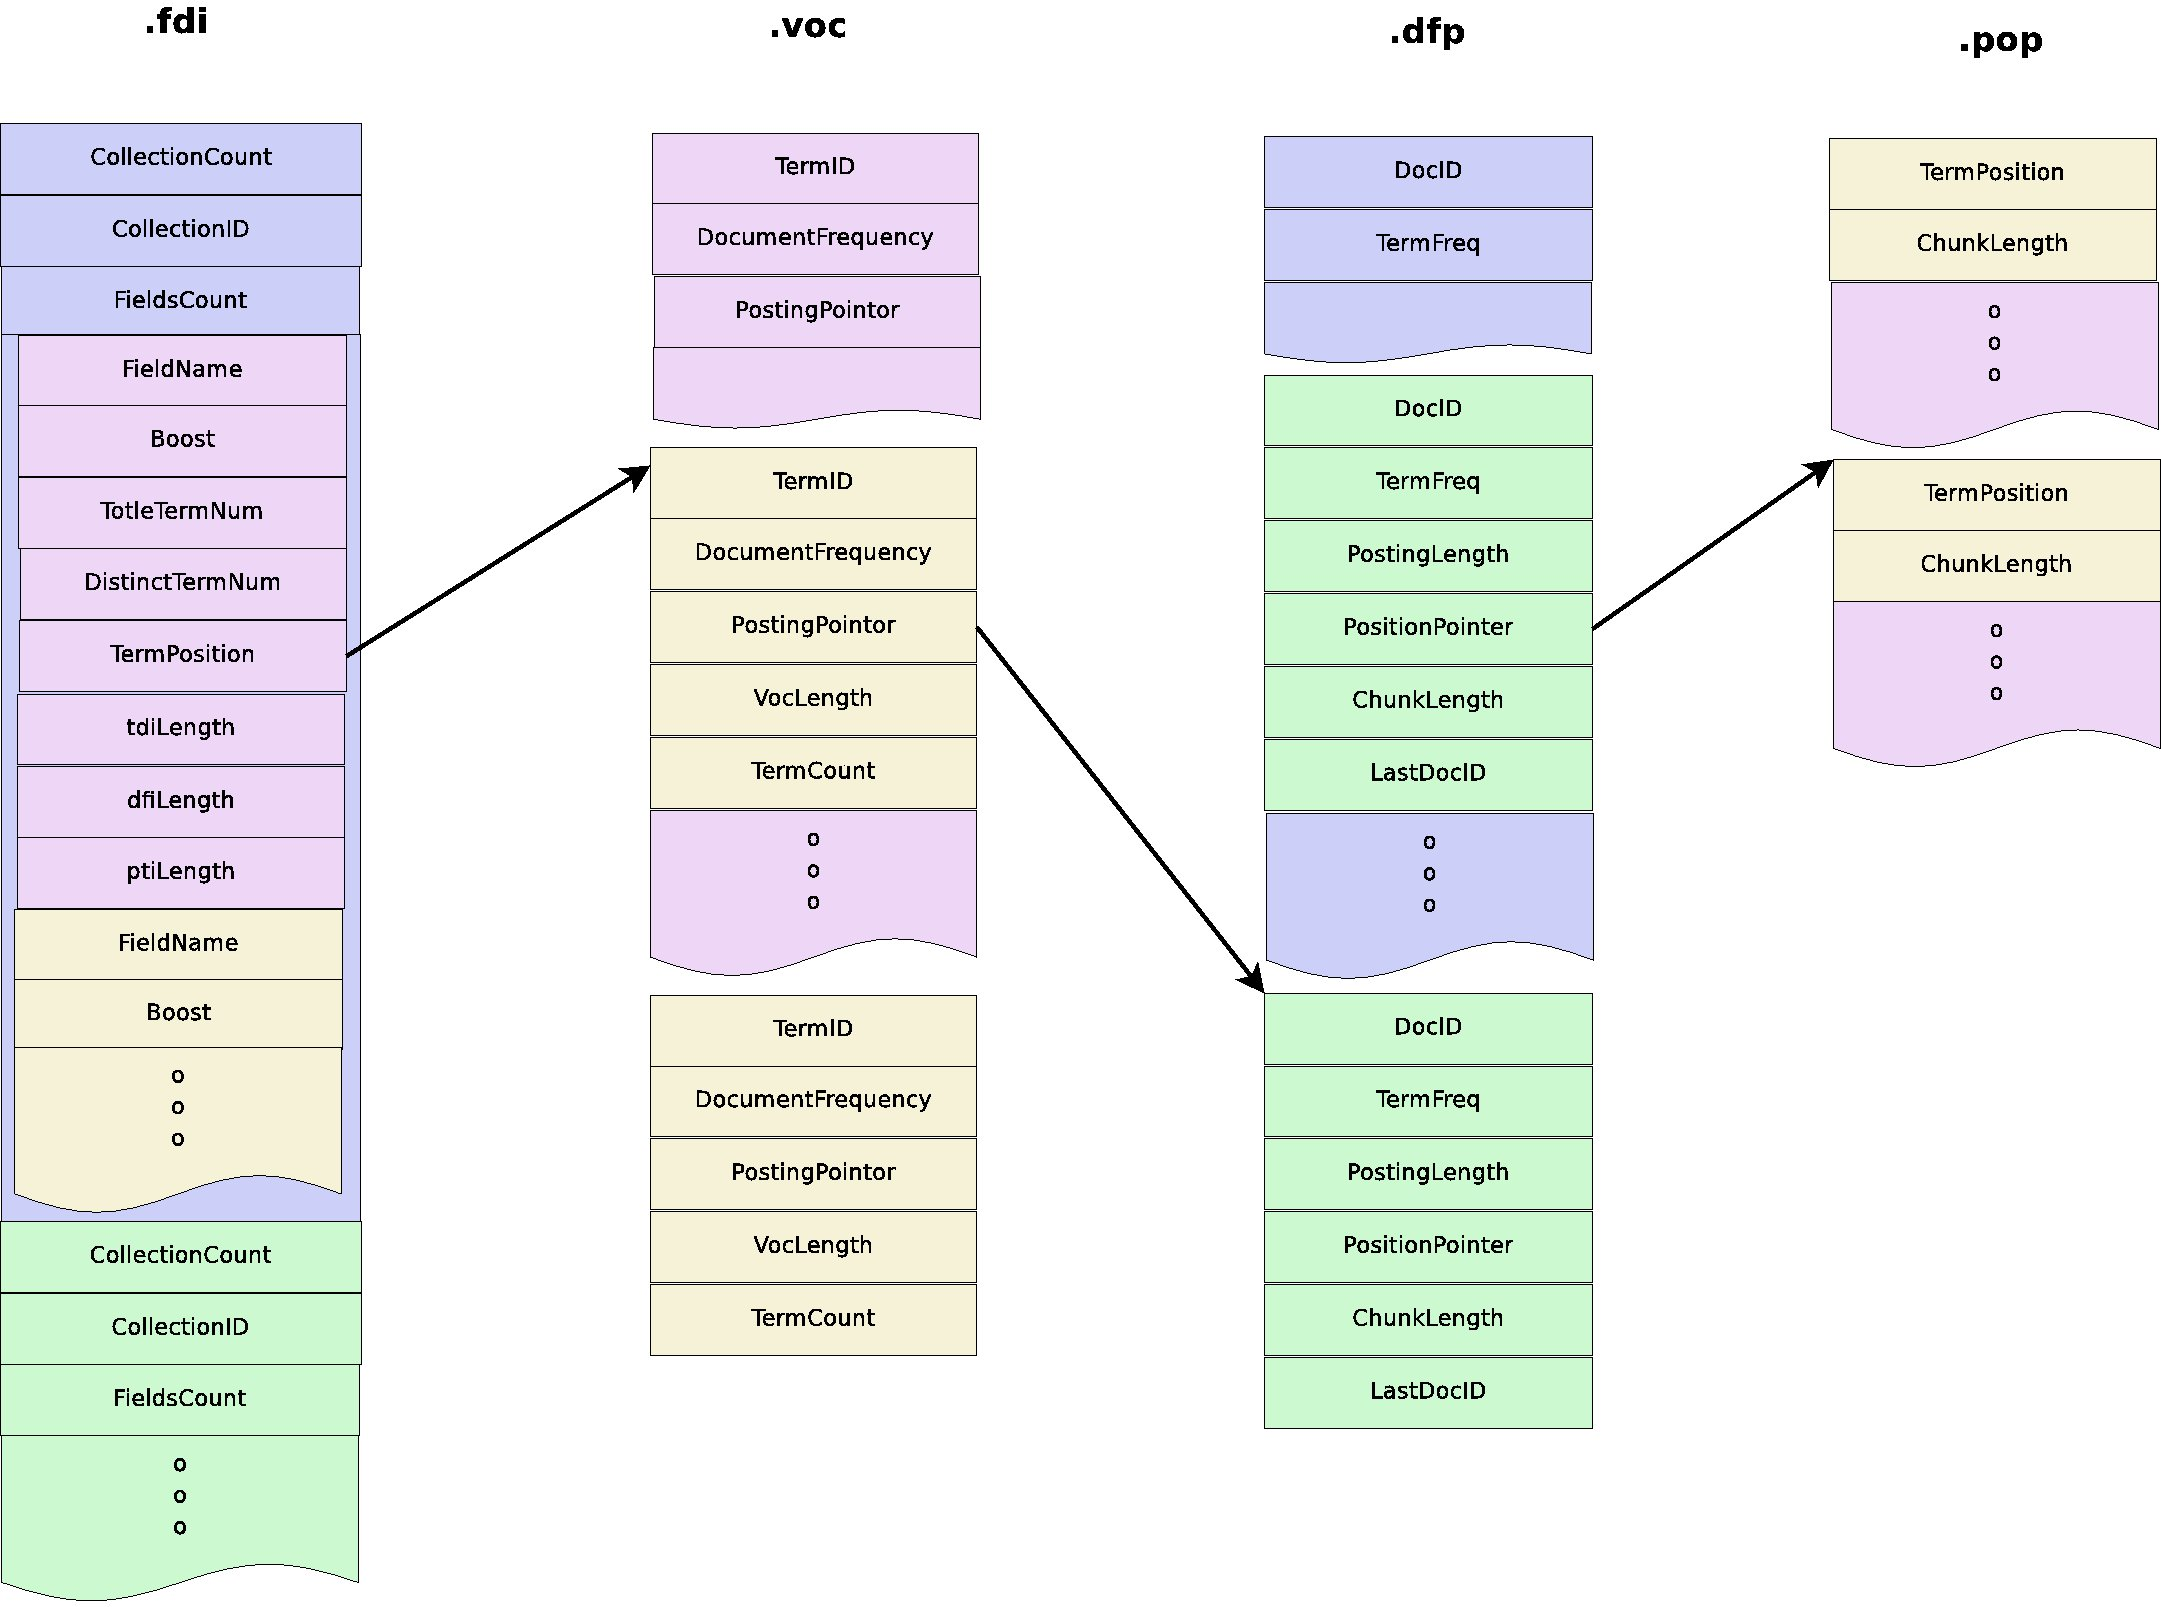
\includegraphics[width= \textwidth]{Figures/barrelFormat.jpg}}
\caption{Index format of a barrel}\label{barrelFormat}
\end{figure}
\par
Let us illustrate these files one by one.

\begin{description}
\item[.fdi] stores information of all fields.

{\scriptsize
\selectfont
\begin{tabular}{ p{.17\textwidth}|p{.06\textwidth}|p{.6\textwidth}}
\textbf{Property} & \textbf{Type} & \textbf{Description}\\
\hline

CollectionCount & Int32 & The count number of collections in this barrel\\
CollectionID & Int32 & The collection id of this collection\\
FieldsCount & Int32 & The count number of fields in this collection\\
FieldName  & string & Field name\\ 
Boost  & Byte  & Boost value of this Field\\
TotalTermNum  & Int64  & Total term number of this Field\\
DistinctTermNum  & Int64  & Total distinct term number of this Field\\
TermPosition  & Int64  & File offset of this Field's vocabulary information in the .voc file\\
tdiLength  & Int64  & Length of this Field's vocabulary information in .voc file\\
dfiLength  & Int64  & Length of this Field's document-frequency postings in the file .dfp\\
ptiLength  & Int64  & Length of this Field's position postings in the file .pop\\

\end{tabular}
}
\item[.voc] vocabulary information of all fields.

{\scriptsize
\selectfont
\begin{tabular}{ p{.17\textwidth}|p{.06\textwidth}|p{.6\textwidth}}
\textbf{Property} & \textbf{Type} & \textbf{Description}\\
\hline
TermID & Int32 & Term ID, it is stored with d-gap encoded.\\
DocumentFrequency & Int32 & The Document frequency, which means how many documents that this term has appeared.\\
PostingPointer & Int64 & File offset of this term's document-frequency posting in the .dfp file\\
VocLength  & Int64 & Same as tdiLength in .fdi\\ 
TermCount  & Int64 & Same as DistinctTermNumin .fdi\\
\end{tabular}
}

\item[.dfp] document-frequency posting.

{\scriptsize
\selectfont
\begin{tabular}{ p{.17\textwidth}|p{.06\textwidth}|p{.6\textwidth}}
\textbf{Property} & \textbf{Type} & \textbf{Description}\\
\hline
DocID               & Int32 & Document ID, which is stored with d-gap encoded.\\
TermFrep            & Vint64 & Term frequency in this document.\\
PostingLength   & Vint64 & Length of this posting\\
PositionPointer  & Vint64 & File offset of the corresponding position posting in the .pop file.\\ 
ChunkLength     & Vint64 & Same as PostingLength\\
LastDocID           & Vint32 & Last document id of this posting.\\
\end{tabular}
}

\item[.pop] position posting.The positions of a term in a document is written in the .pop file sequentially.

\end{description}
\par



\subsection{IndexMerger}

IndexMerger takes charge of merging multiple index barrels if the merge conditions are satisfied. When a merge event happens, all the barrels that are needed to be merged are ordered according to the document number that each barrel has contained, then the merging process will be proceeded field by field. FieldMerger is responsible for merging same field of a collection in different barrels, and PostingMerger will merge postings at the term level.

\begin{figure}[htb]
\centerline{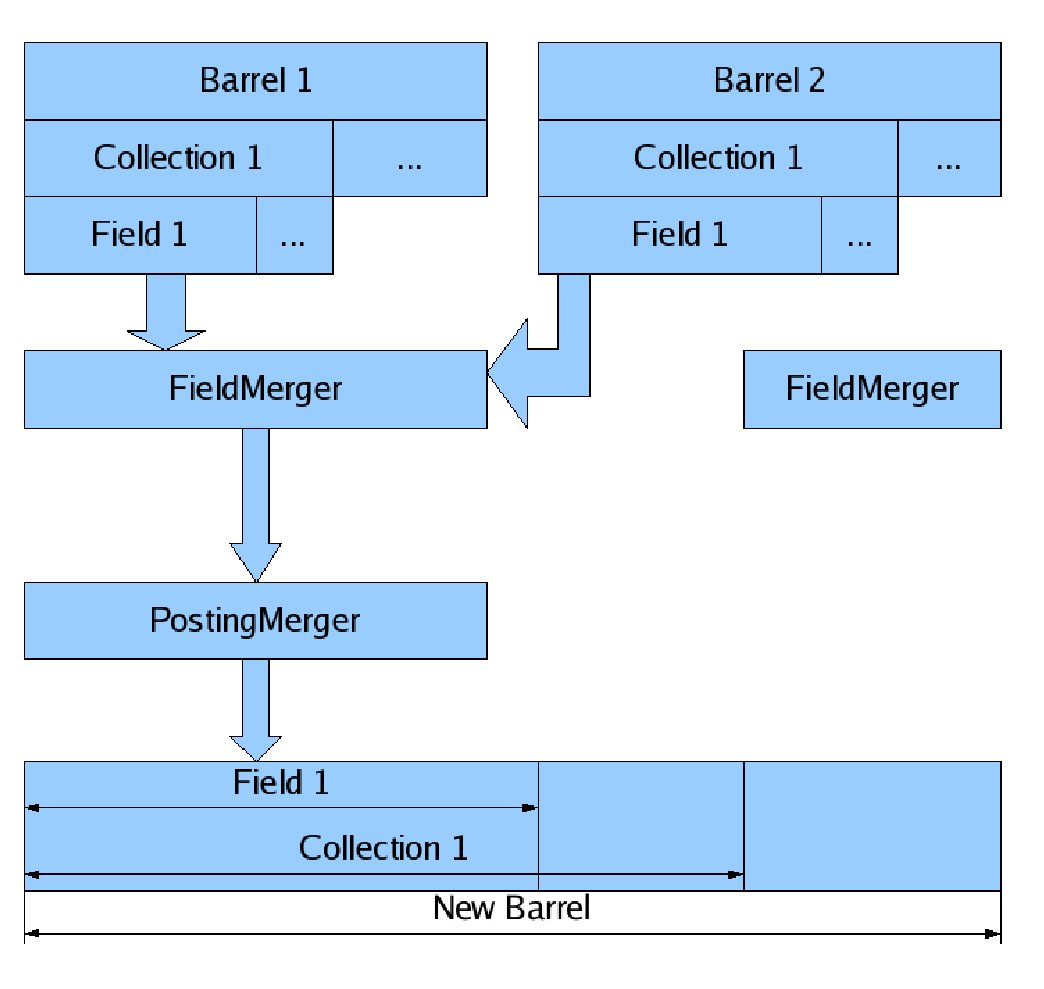
\includegraphics[width=0.4\textwidth]{Figures/indexmanager.jpg}}
\caption{Hierarchy of IndexMerger}\label{indexmanager}
\end{figure}

IndexMerger could be configured to run within a stand-alone thread, in that case, there exist complicated index sychronization mechanism between IndexMerger and IndexReader, because IndexMerger will remove old index barrels after a successful merge, while the IndexReader can not always check the validation due to the performance of searching.


\subsection{IndexReader}


\begin{figure}[h!]
\centerline{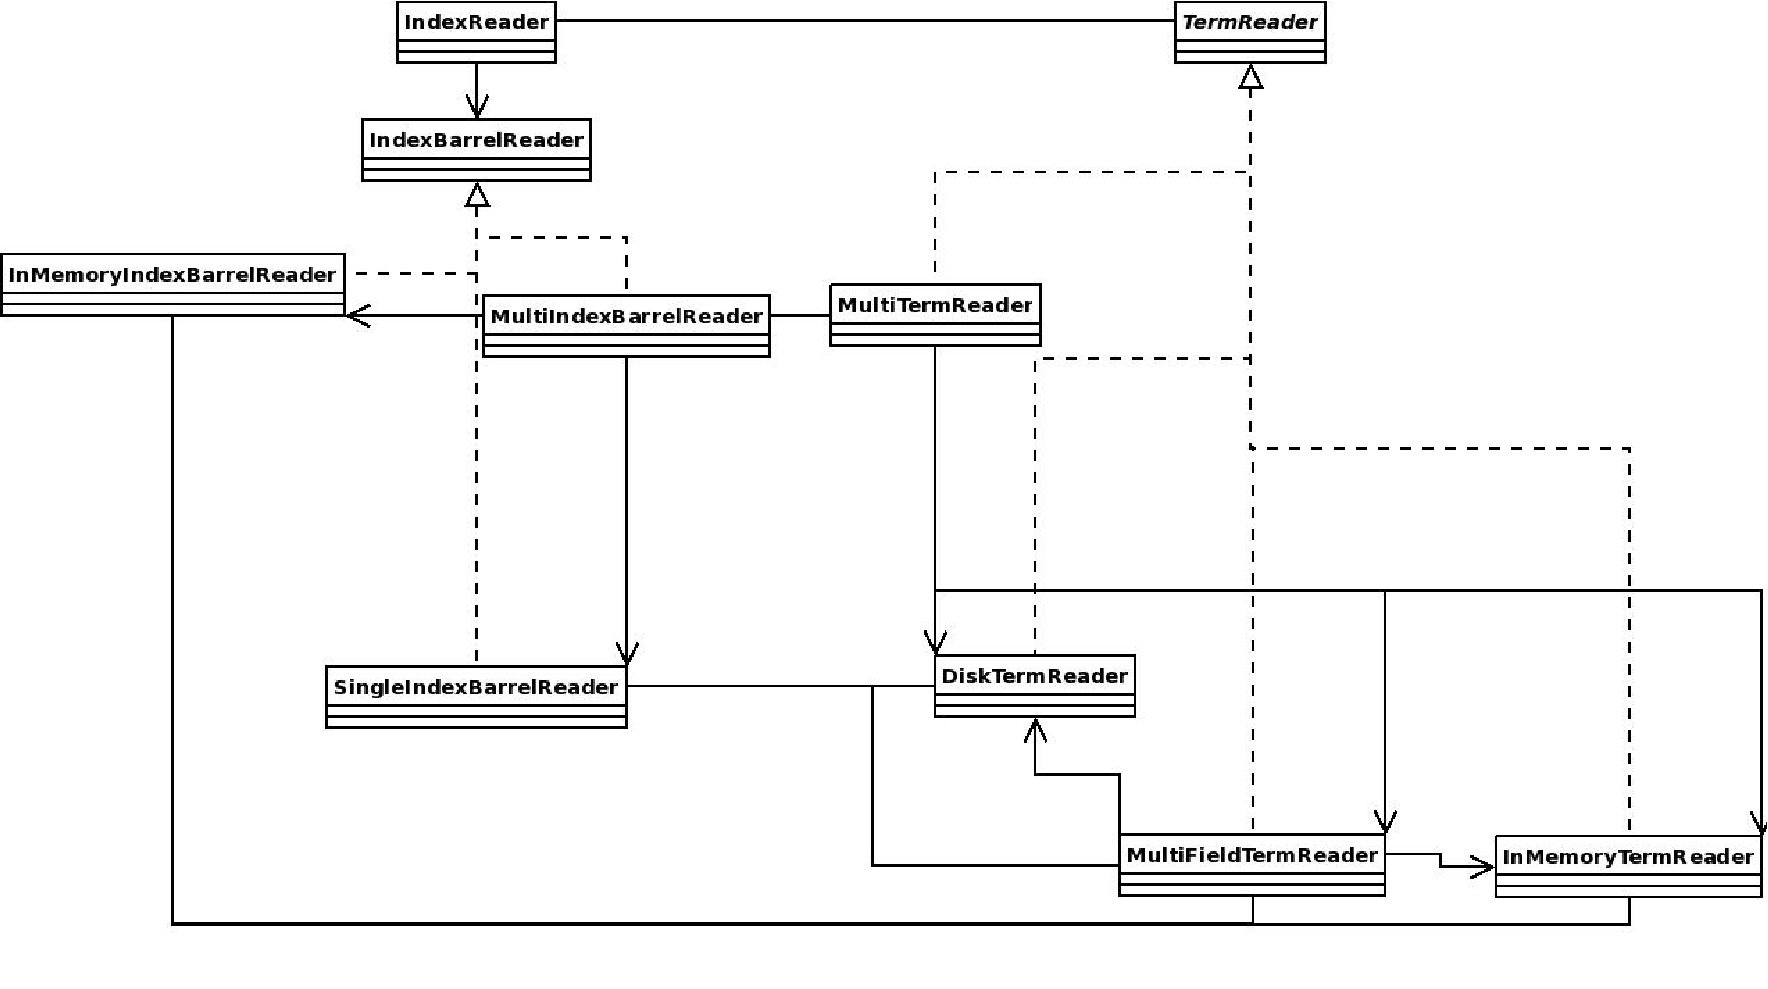
\includegraphics[width=\textwidth]{Figures/indexreader.jpg}}
\caption{Components of IndexReader}\label{indexReader}
\end{figure}


\par
IndexReader is the interface to read inverted indexes and search them. Figure \ref{indexReader} gives a detailed class diagram of the components of IndexReader. When IndexReader is created, it will open the index barrels and return an instance of TermReader to users. TermReader takes charge of seeking a term in the vocabulary of the indexes, and then iterating its corresponding posting list according to the user's requests. SingleIndexBarrelReader is used to open a single index barrel and return its TermReader, here it is the DiskTermReader. Because IndexManager should support on-line indexing, which means the indexes could be searched during index construction, therefore, those indexes that have not been flushed to disk should also allow being searched, InMemoryIndexBarrelReader takes this responsibility. What's more, since there may exist several barrels in the system, then we have MultiIndexBarrelReader which contains several instances of SingleIndexBarrelReader or InMemoryIndexBarrelReader, each of which 
takes charge of reading their corresponding sub-index. Accordingly,  the TermReader got by InMemoryIndexBarrelReader should be InMemoryTermReader, and the TermReader got from MultiIndexBarrelReader should be MultiTermReader, which is composed of several instances of DiskTermReader and InMemoryReader similarly.

\par
After getting an instance of TermReader, the user could use it to search the inverted indexes: if the term to be queried could be found by TermReader in the indexes, then TermReader could return an index iterator TermDocFreqs or TermPositions. Just as Figure \ref{indexmanager} shows. TermDocFreqs will iterate the document-frequent postings and TermPositions will iterate document-frequent postings and position postings both, therefore TermPositions is inherited from TermDocFreqs. They are the major search utilities interface classes exposed to users.\par

\begin{figure}[h!]
\centerline{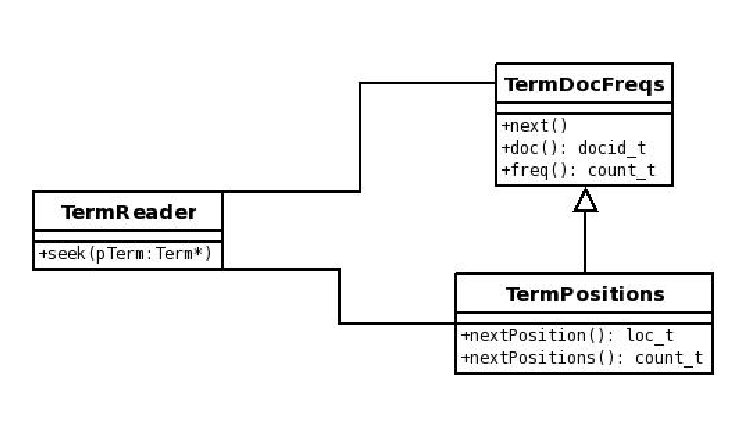
\includegraphics[width=0.5\textwidth]{Figures/termPos.jpg}}
\caption{TermDocFreqs and TermPositions}\label{termPos}
\end{figure}


\subsection{Search Optimization}
Search performance is always the most important design issue for index design. We have two approaches for search optimization:

\subsubsection{Embedded Skiplist}
Embedded skip list is used to accelerate conjunction operation of multiple posting lists. Suppose we have two postings that contain doc ids:
\begin{lstlisting}[language=C]
1,2,3,4,10,11,100,120,1000,...

1,10,1000,...
\end{lstlisting}
The conjunction operation for these two postings should be: $1,10,1000,...$ . For index without embedded skiplist, we must read and decompress all posting data, while if we have implemented skiplist within posting list,
we could use these operations to avoid of frequent disk IO:
\begin{lstlisting}[language=C]
  pDocIterator->skip(10);
  pDocIterator->skip(1000);
\end{lstlisting}

The assumptions for the embedded skiplist are:
\begin{itemize}
 \item Seeking forward to a certain place will take less time than read. In the above example: it means within the first posting, the time taken by the file seek operation from doc id of 1 to doc id of 10, is less than the time 
taken by reading all posting data between those two doc ids.  This is especially true for conjunction operation over short posting list and long posting list.
 \item Document ids within each posting list should be an incremental order. 
\end{itemize}

Figure \ref{skiplist} shows the detailed design for an embedded skiplist---For simplicity, it has not contained the information of term position posting lists:
\begin{figure}[h!]
\centerline{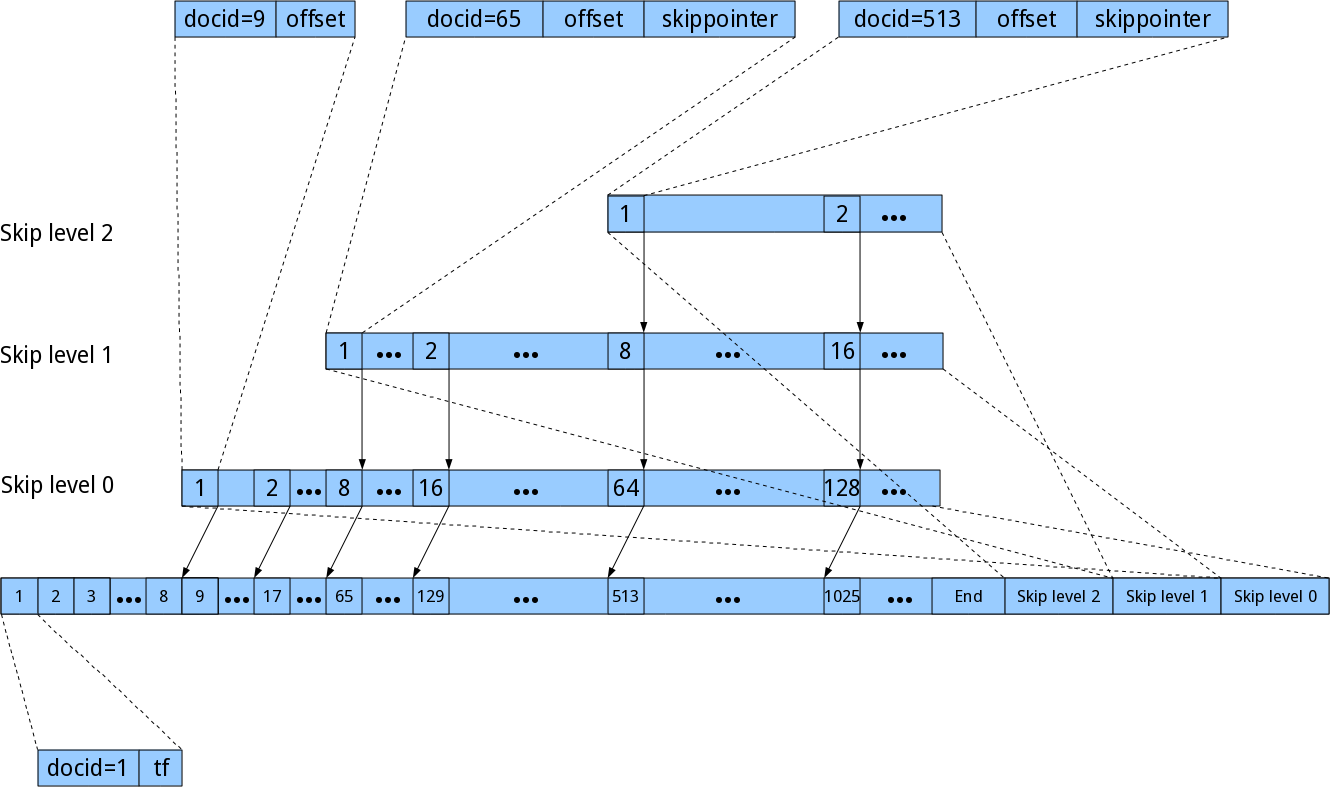
\includegraphics[width=0.8\textwidth]{Figures/skip.png}}
\caption{Embeded SkipList Design}\label{skiplist}
\end{figure}

Several points are needed to be illustrated:
\begin{itemize}
 \item In this example, we have embedded a skiplist with an interval of 8 and a max skip level of 3. Which means, during indexing, we will record a skip point every 8 documents. The skip interval of the second skip level is $8*8=64$,
while the skip interval of the upmost skip level is $8*8*8=512$.
 \item Each skip point contains two kinds of data:
   \begin{enumerate}
    \item Current skipped document id.
    \item File offsets of skipped point, including both \texttt{dfp} posting list and \texttt{pos} posting list.
   \end{enumerate}
 \item We should consider the location of skiplist data. In the example graph, the skiplist data locates at the end of each posting. It is very convenient for posting merging, because skiplist data will not be generated until the overall posting
list is merged, if we put skiplist data at the end of each posting, we could directly write skip data just after merging postings.  However, such design will hurt the query performance---it will lead to file seek operations not sequential
any more. Therefore, with the eventual implementation, the skiplist data is put at the head of each posting---In this case, it's pretty inconvenient for posting merge operation, we will discuss this issue in the following part.
\end{itemize}

Figure \ref{skiplist-merge} illustrates the design issue for posting merge when we have added embedded skiplist data to index. From the upper part of this graph we can see the posting merge is pretty direct, while if we put skiplist data
at the beginning of the posting list, it will introduce more complicated design: During merging operation, we could directly write the skiplist data of merged posting to the index file, while we need an extra intermediate file to store the 
merged posting data. After all posting merging is finished, we should copy data from that intermediate file to index file. Only through this operation could we provide skip list data at the beginning of each posting.

\begin{figure}[h!]
\centerline{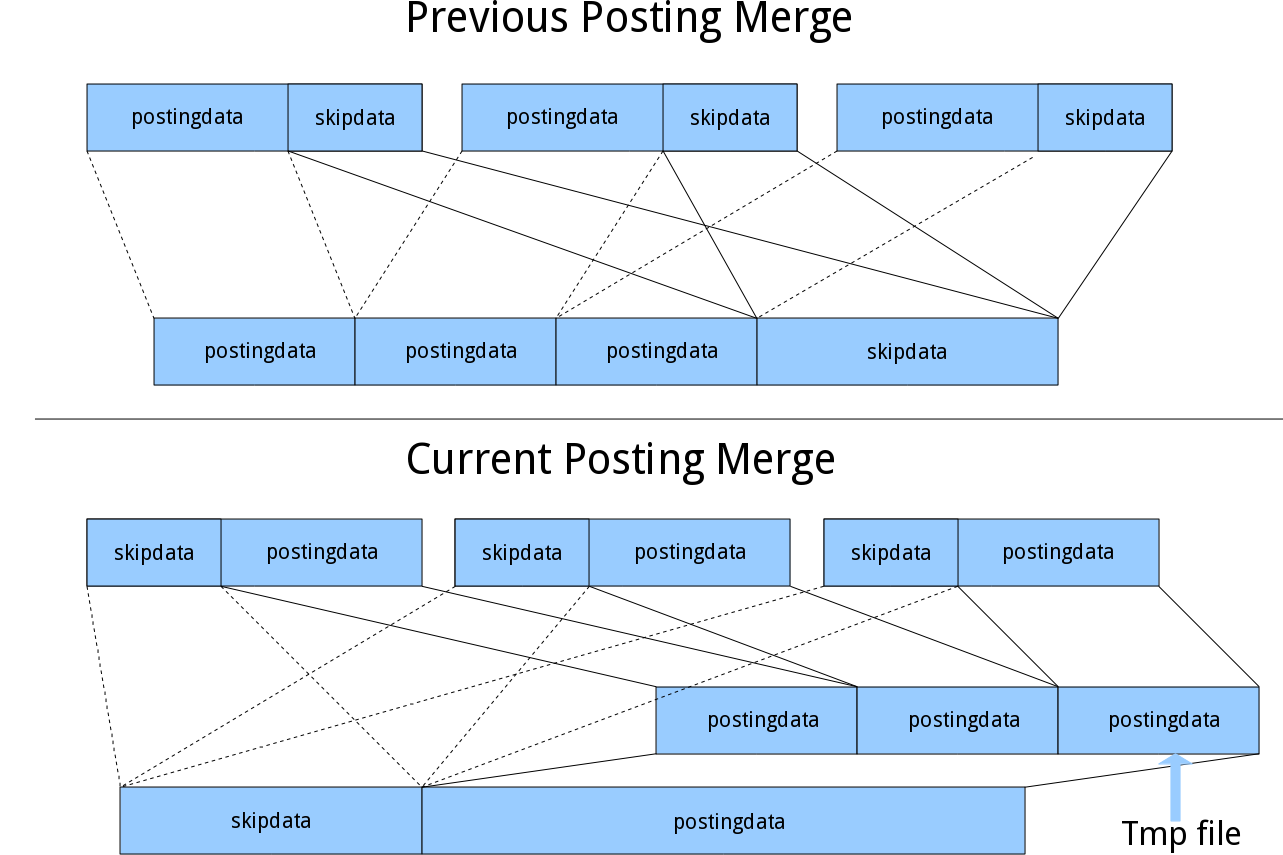
\includegraphics[width=.8\textwidth]{Figures/skipmerge.png}}
\caption{Posting Merge With SkipList}\label{skiplist-merge}
\end{figure}


Another design issue for skiplist design is also caused by the posting merge, seen from figure \ref{skiplist-interval}:
\begin{figure}[h!]
\centerline{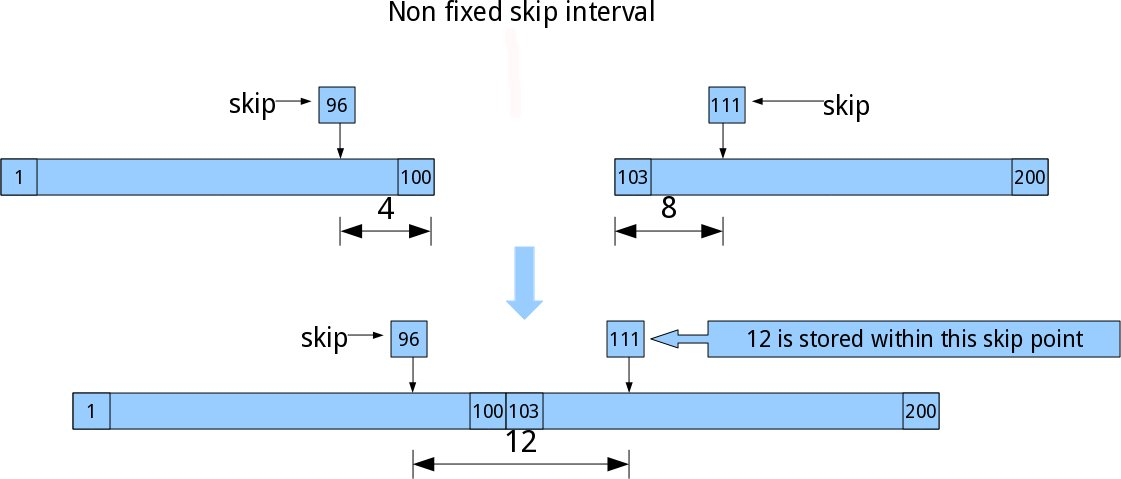
\includegraphics[width=.8\textwidth]{Figures/skipinterval.jpg}}
\caption{Unfixed Skip Interval Design}\label{skiplist-interval}
\end{figure}

In this example, both two posting have a skip interval of 8. However, at the end of the first posting, there are only 4 documents left, as a result, after merging these two postings, the skip interval between document $96$ and
document $111$ should have to be reconsidered:
\begin{itemize}
 \item One solution is to still keep the fixed skip interval. In this case, all skip data will have to be regenerated after posting merging.
 \item The other solution is to introduce unfixed skip interval. In this case, the skipinterval between document $96$ and document $111$ will be 12 instead of 8 any more.
\end{itemize}

IndexManager adoptes the second solution, because it requres less operation for merging skiplist data. Obviously, it introduce extra storage overheads because we have to record skip interval value for certain skip points.

\subsubsection{New Compression}
New compression is another approach for search optimization. Due to the fact that all of the cutting-edge compression schemes are totally different with general variable byte length based solution, IndexManager must provide a 
good abstraction so that all kinds of index format can be supported and switched easily just by a configuration parameter. Shown in figure \ref{newindexclass}, the basic abstraction is \texttt{PostingWriter} and \texttt{PostingReader}.
They are two interface classes owned by IndexWriter and IndexReader. We provide new compression based index within \texttt{EPostingWriter} and \texttt{EPostingReader}.

\begin{figure}[h!]
\centerline{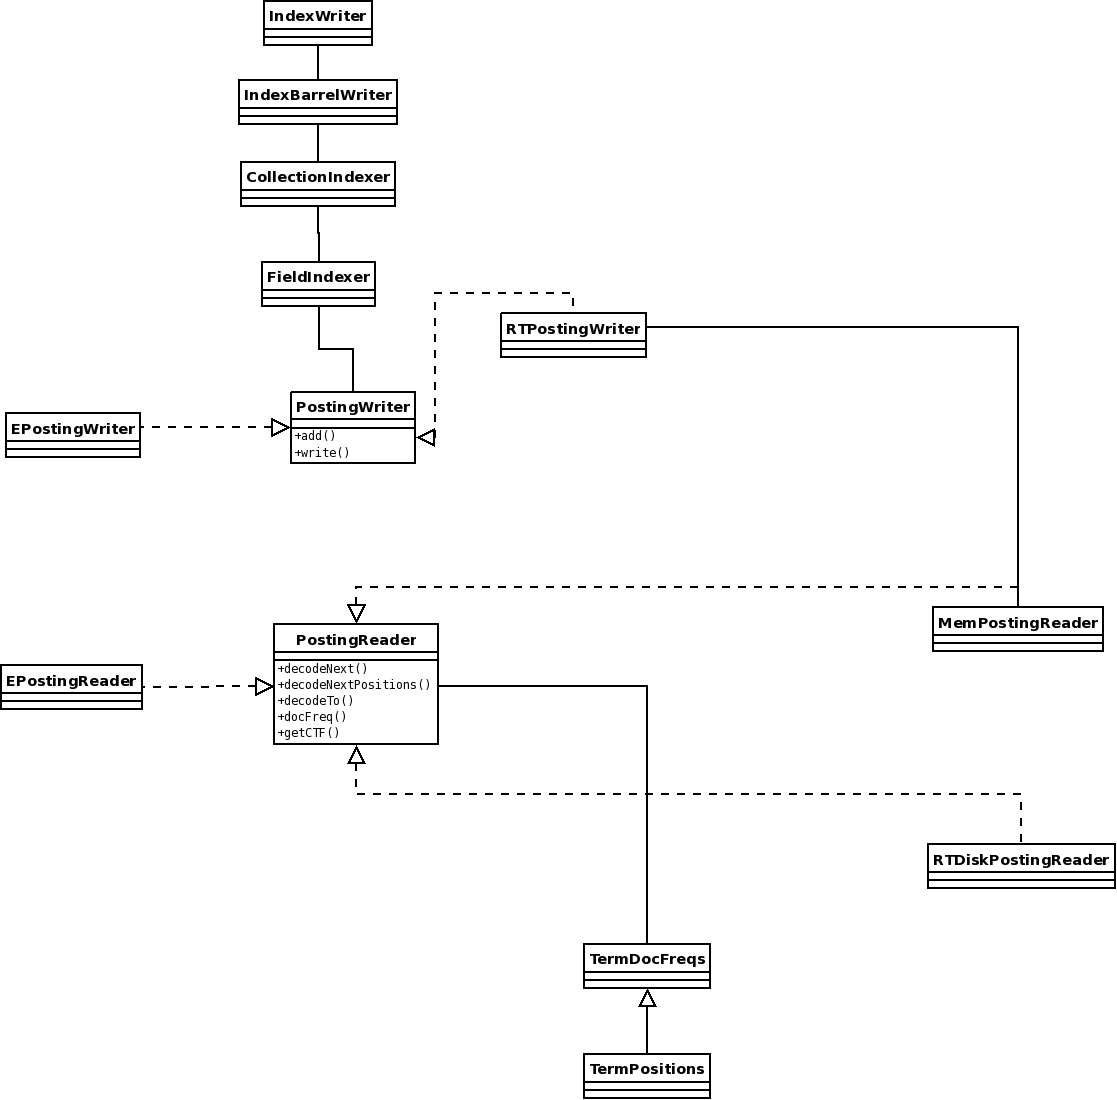
\includegraphics[width=.8\textwidth]{Figures/newindexclass.png}}
\caption{Class Diagram Overview For New Index}\label{newindexclass}
\end{figure}


In order to be flexible enough to switch among all the new compression schemes, IndexManager provides a wrapper class:

\begin{lstlisting}[language=C]
template<typename PrimaryCompressor>
struct CompressorType
{
    int compress(uint32_t* input, uint32_t* output, int num_input_elements) const;

    int decompress(uint32_t* input, uint32_t* output, int num_input_elements) const;
};
\end{lstlisting}

So that if we want to change the compression scheme, we just need to redefine cooresponding template parameters:

\begin{lstlisting}[language=C]
typedef CompressorType<PForDeltaMix_Compressor> DocIDCompressor;

typedef CompressorType<S16_Compressor> TermFreqCompressor;

typedef CompressorType<S16_Compressor> TermPosCompressor;
\end{lstlisting}


Before illustrating how the new compression schemes are used within index, let us first describe how those compression approaches work at first:
\begin{enumerate}
 \item Variable-Byte Coding: Variable-byte compression represents an integer in a variable number of bytes, where each byte consists of one
status bit, indicating whether another byte follows the current one, followed by 7 data bits. Variable-byte compression does not achieve a very
good compression ratio, but is simple and alows for fast decoding, as a result, it is the most popular compression solution in existing IR frameworks.
 \item S9: Simple9 coding is an algorithm proposed in \cite{anh2005inverted} that combines good compression and high decompression speed. The basic
idea is to try to pack as many values as possible into a 32-bit word. This is done by dividing each word into 4 status bits and 28 data bits, where the
data bits can be partitioned in 9 different ways. For example, if the next 7 values are all less than 16, then we can store them as 7 4-bit values. Or
if the next 3 values are less than 512, we can store them as 3 9-bit values(leaving one data bit unused).

Simple9 uses 9 ways to divide up the 28 data bits: 28 1-bit numbers, 14 2-bit numbers, 9 3-bit numbers(one bit unused), 7 4-bit numbers, 5 5-bit numbers
(three bits unused), 4 7-bit numbers, 3 9-bit numbers(one bit unused), 2 14-bit numbers, or 1 28-bit numbers. The 4 status bits store which of the 9 cases
is used. Decompression can be optimized by hardcoding each of the 9 cases using fixed bit masks, and using a switch operation on the status bits to select the case.
 \item S16: Simple16 \cite{zhang2008performance} uses the same basic idea as S9, but has 16 ways of partitioning the data bits, where each of the 16 cases uses 
all of the 28 data bits. The result is that S16 approximately matches the speed of S9, while achieving slightly better compression. 
 \item PForDelta: This is a compression method recently proposed in \cite{zukowski2006ssr} that supports extremely fast decompression while also 
achieving a small compressed size.  PForDelta first determines a value $b$ such that most of the values to be encoded(say, $90\%$) are less than $2^b$ and thus
fit into a fixed bit field of $b$ bits each. The remaining values, called $exceptions$, are coded separatedly.  If we apply PForDelta to blocks containing some multiple
of 32 values, and finally patching the result by decoding a smaller number of exceptions. This process can be implemented extremely efficiently by providing,
for each value of $b$, an optimized method for extracting 32 b-bit values from $b$ memory words. PForDelta can be modified and tuned in various ways by choosing
different thresholds for the number of exceptions allowed, and by encoding the exceptions in different ways.

Within IndexManager, the composite compression scheme that uses variable-byte approach to compress the exceptions is names as \texttt{PForDeltaMix} compressor.
From the research work in \cite{yan2009compressing}, another improvements for PForDelta have been presented: Recall that the implementations of PForDelta 
in previous work encode a block of 128 value by first allocating 128 b-bit slots, and then for those $90\%$ of the values less than 2b directly storing them in their 
corresponding slots. For each value larger than 2b , called a exception, we store an offset value in the exception's corresponding slot indicating the distance from 
the current exception to the next one, and the actual value of the exception in some additional space after the 128 b-bit slots. One disadvantage of such a code 
structure is that when two consecutive exceptions have a distance of more than 2b , we have to use more than one offset to represent the distance, by forcing 
additional exceptions in between these two exceptions. We cannot solve this problem by simply increasing b since this would waste lots of bits on $90\%$ of values; 
but if we decrease b more exceptions will be produced. This means in particular that this version of PForDelta cannot profitably use any values of b less than b = 3.
To overcome this problem, they present a new code structure for PForDelta that stores the offset values and parts of the exceptions in two additional arrays. 
In particular, for an exception, they store its lower b bits, instead of the offset to the next exception, in its corresponding b-bit slot, while they store the higher overflow
bits and the offset in two separate arrays.  These two arrays can be further compressed by any compression method, and they find that S16 is particularly suitable for
this. Another improvement is in the selection of the b value for each block. As it turns out, selecting a constant threshold for the number of exceptions does not 
give the best tradeoff between size and speed. Instead, they model the selection of the b for each block as an optimization problem: initially assign the b with the
smallest compressed size to each block, and then increase speed as desired by selecting a block that gives us the most time savings per increase in size, and change the b 
of that block. For a given target speed, we can easily derive simple global rules about the choice of b, instead of running the iterative optimization the above. Thus this 
version can be very efficiently implemented even on very large collections.

\par
Within IndexManager, we call this composite compression scheme PForDelta-Mix-S16 compressor. According to the description above, the optimization procedure for choosing
best b value takes longer time---around 10 times longer than general PForDelta according to the experiments, while it can achieve more benefits during search operations. 
\end{enumerate}

Based on the above template wrapper for compressor, as well as a suit of compression schemes, such as: S16, PForDelta, PForDeltaMix, PForDeltaMixS16, ..., etc, we provide
two kinds of index format within which any of the new compression scheme could be applied, shown in figure \ref{newindex}:

\begin{figure}[h!]
\centerline{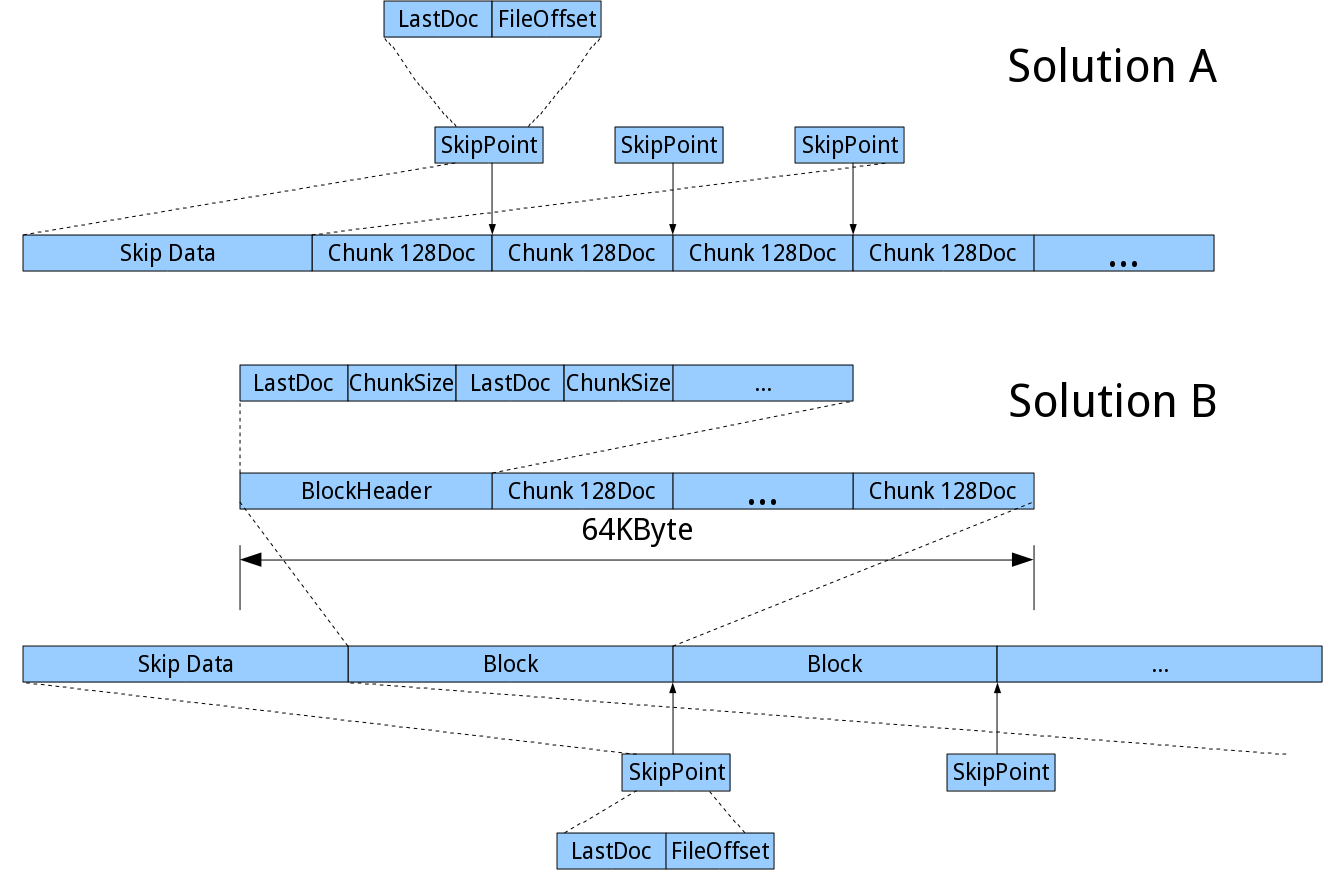
\includegraphics[width=.8\textwidth]{Figures/newindex.png}}
\caption{Chunk and Block Type Index}\label{newindex}
\end{figure}

\begin{itemize}
 \item \texttt{Chunk Type}---solution A in figure \ref{newindex}\par
Chunk type index directly compress posting data for every 128 documents, and we call each compression unit with the terminology $chunk$. The embedded skiplist data is totally 
the same with the original index, with a fixed skip interval of 128.

 \item \texttt{Block Type}---solution B in figure \ref{newindex} \par
The idea of block type index comes from the requirements that disk IO performs the best for a fixed block of size. In this design, the posting data is partitioned into a series of
block each of which has a fixed size, say, 64K bytes. Within each block, there are a series of chunk that contains posting data for every 128 documents. There are several
benefits for block type index over chunk type:
\begin{enumerate}
 \item It is very easy to provide posting level cache based on block type index. \par
Given a large scale web search system, we need to set up multi level cache mechanism to support huge search requests. Posting level cache is always the lowest level and the most
difficult to design. However, having block type index, implementing such cache is much easier: we just need to record each block identifier and store them into cache.
 \item We could provide more compression to posting data: \par
When implementing chunk type index, besides the chunk that contains posting data for every 128 documents, we still need to store these values to posting list:
\begin{itemize}
 \item Size of each chunk. Generally, it is stored using variable byte compression.
 \item Skip data, containing current skip doc id and file offsets. They are also stored using variable byte compression.
\end{itemize}
With block type index, we only need to set up an embedded skip list for blocks, while within each block, we have block header data that contains size and last doc id for each chunk,
these data are put together so we could use another better compressor to compress block header data.

The weakness for block type index is also remarkable: It supposes each posting list would occupy at least one block. For smaller corpus, most of the index contains useless data.
So block type index is more suitable to serve as extremely large index, especially for supporting web search, while chunk type index is more general.  
\end{enumerate}
 
\end{itemize}


There are two more design issues caused by the new compression scheme:
\begin{itemize}
 \item Location of term position posting data. \par
Just the as the original variable byte length based index, the term position posting data is still put into another file, instead of putting together with doc ids and term frequencies, shown
in figure \ref{termpos-chunk};

\begin{figure}[h!]
\centerline{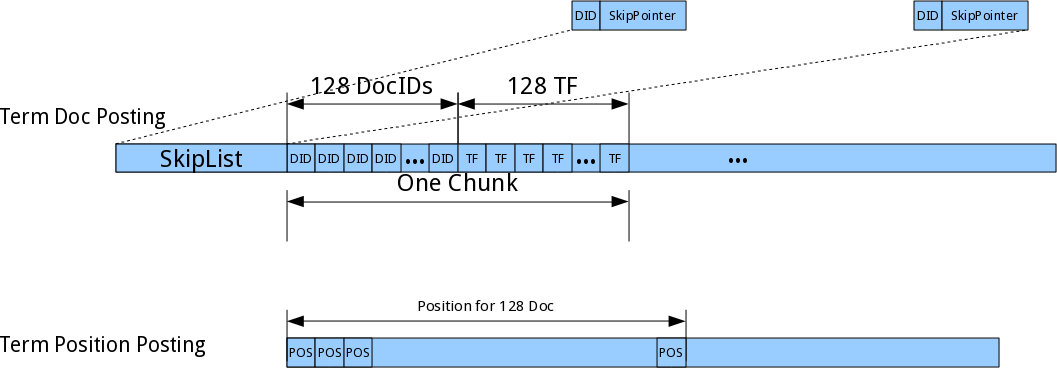
\includegraphics[width=.8\textwidth]{Figures/termpos.png}}
\caption{Term Position Data for Chunk Type Index}\label{termpos-chunk}
\end{figure}

We design in this way just for better reusage for existing IndexManager components.
 \item Posting merge issue. \par
Another design issue is caused by posting merge. No matter chunk type or block type index, all of them compress posting data in a batch way with fixed documents. When merging two 
postings, suppose the last chunk for the first posting only contains posting data for 21 documents, we can only have two choices to deal with such kinds of data chunk:
\begin{enumerate}
 \item Decompress all posting data of the second posting, then recompress them together with the data from the first posting.
 \item For every chunk, do not compress data from a fixed size of documents.
\end{enumerate}
IndexManager has adopted the first choice, because the other approach has introduced more overheads---it will cause the inefficiency of PForDelta based compression scheme. 
As a result, given that either of chunk type or block type index is adopted, we should have a much slower merging performance, both of these two kinds of index should be chosen according
to practical situations.
\end{itemize}

